%\documentclass[11pt]{amsart}
\documentclass{amsbook}
\usepackage{geometry}                % See geometry.pdf to learn the layout options. There are lots.
\geometry{letterpaper}                   % ... or a4paper or a5paper or ... 
%\geometry{landscape}                % Activate for for rotated page geometry
%\usepackage[parfill]{parskip}    % Activate to begin paragraphs with an empty line rather than an indent
\usepackage{graphicx}
\usepackage{amssymb}
\usepackage{bbold}
\usepackage{epstopdf} % for double-one identity matrix, \mathbb{1}.
\usepackage{myMacros}
\DeclareGraphicsRule{.tif}{png}{.png}{`convert #1 `dirname #1`/`basename #1 .tif`.png}

\title{Nodal FEM Notes}
\author{Paul Hansen}
%\date{}                                           % Activate to display a given date or no date

\begin{document}
\maketitle

\tableofcontents
\chapter{Preliminaries}
\label{chap:preliminaries}

\section{Basic things}

Following \cite{hesthaven2007nodal}, define orthonormal basis functions $\phi_1, \phi_2, \cdots, \phi_N$ and nodes $\ve r_1, \ve r_1, \cdots, \ve r_N$ on the reference element.

A function $u(\ve r)$ in the space spanned by the basis functions can be uniquely given by its modal coefficients $\hat{u}_1, \cdots, \hat{u}_N$ or by its nodal values $u(\ve r_1), \cdots, u(\ve r_N)$.  The Vandermonde matrix $V_{ij}$ converts modal coefficients to nodal values,
%
\begin{equation}
\boxed{
V = \begin{bmatrix} \phi_1(\ve r_1) & \phi_2(\ve r_1) & \hdots & \phi_N(\ve r_1) \\
\phi_1(\ve r_2) & \phi_2(\ve r_2) & \hdots & \phi_N(\ve r_2) \\
\vdots & \vdots & \ddots & \vdots \\
\phi_1(\ve r_N) & \phi_2(\ve r_N) & \hdots & \phi_N(\ve r_N)
\end{bmatrix}
}
\end{equation}
%
so that $u(\ve r_i) = V_{ij} \hat{u}_j$.

To evaluate a function at non-nodal points we use the Vandermonde matrix and the values of the basis functions at the evaluation points.
%
\begin{equation}
u(r') = \hat{u}_i \phi_i(r') = \ve{u}^T V^{-T} \begin{bmatrix} \phi_1(r') \\ \phi_2(r') \\ \vdots \\ \phi_N(r') \end{bmatrix}.
\label{eqn:interpolation}
\end{equation}

\section{Integration and differentiation on the reference element}

\subsection{Quadrature}

Because the basis functions are orthonormal on the reference element, the Vandermonde matrix can be used for quadrature of functions sampled on nodal points\footnote{Let's go ahead and assume that all functions such as the examples $f(\ve r)$ and $g(\ve r)$ are sums of the basis functions so quadrature is exact.}:
%
\begin{equation}
\int_\bigtriangleup dr \, f(\ve r) g(\ve r) = f(\ve r_i) (V^{-1})_{ji}(V^{-1})_{jk} g(\ve r_k) = \ve f^T V^{-T} V^{-1} \ve g
\end{equation}
%
in various notations.  We define the reference element inner product kernel
%
\begin{equation}
\boxed{
Q = V^{-T} V^{-1}
}
\end{equation}
%
and note that quadrature can be carried out with the kernel $\ve 1^T Q$:
%
\begin{equation}
\int_\bigtriangleup dr \, f(\ve r) = \ve 1^T Q \ve f.
\end{equation}

\subsection{Differentiation}

The gradient of the Vandermonde matrix is calculable from gradients of the basis functions.  The gradient of a function at the nodal points is calculable by decomposing it into basis functions, differentiating them and summing them back up.  Without loss of generality take the derivative in the $r$ direction:
%
\begin{equation}
\boxed{
D_r = \pp{V}{r} V^{-1}
}
\end{equation}
%
\begin{equation}
\renewcommand\arraystretch{1.5}
\begin{bmatrix}
\pp{f}{r}(\ve r_1) \\ \pp{f}{r}(\ve r_2) \\ \vdots \\ \pp{f}{r}(\ve r_N)
\end{bmatrix}
=
D_r \begin{bmatrix} f(\ve r_1) \\ f(\ve r_2) \\ \vdots \\ f(\ve r_N) \end{bmatrix}.
\end{equation}

\section{Coordinate transformations}

Coordinate transformations are ubiquitous in FEM because the elemental equations are all transformed versions of the elemental equations on a single reference element.  For unstructured meshes of triangles or tetrahedra of different sizes and orientations, the governing equations are all ultimately formulated on the reference element.  Curvilinear elements, arising from non-affine coordinate transformations, are particularly gross.

When directly differentiating the FEM system for sensitivity analysis, the sensitivity of the Jacobian plays the central role.  We'll get there too.

\subsection{Transforming the 2D reference element}

Following \cite{hesthaven2007nodal}, take the basis element to be a simplex with vertices $(r,s) = \left\{ (-1,-1), (1,-1), (-1,1) \right\}$ (Fig. \ref{fig:reference_simplex}).
%
\begin{figure}[!ht]
\centerline{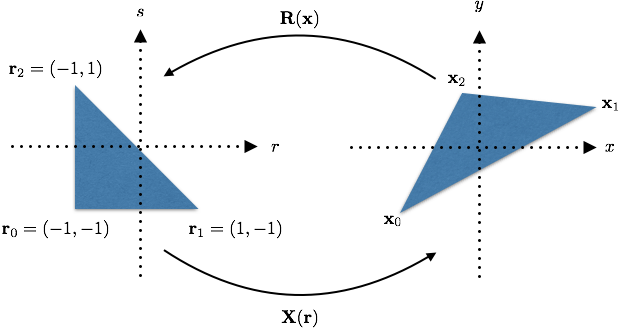
\includegraphics[width=7cm]{reference_simplex.png}}
\caption{The reference simplex (left) and its transformed version (right).  The coordinate transformation $\ve X(\ve r)$ maps $\ve r_0 \mapsto \ve x_0$, $\ve r_1 \mapsto \ve x_1$, and $\ve r_2 \mapsto \ve x_2$.  $\ve{X}(\ve{r})$ and $\ve{R}(\ve{x})$ are inverses of each other.}
\label{fig:reference_simplex}
\end{figure}
%
Points $\ve r = (r,s)$ in the reference simplex are mapped to $\ve x = (x,y)$ in each finite element by the per-element coordinate transformation $\ve X(\ve r; \ve p)$.  The transformation depends on the design parameters $\ve p$ because changing $\ve p$ may change the shapes of structures in the simulation and thus change the mesh.  The mapping $\ve R(\ve x; \ve p)$ is defined as the inverse of $\ve X$, so that for fixed $\ve p$,
%
\begin{equation}
\ve R(\ve X(\ve r; \ve p); \ve p) = \ve r.
\end{equation}
%
Integrals in $(x,y)$ space are performed in $(r,s)$ coordinates to take advantage of the axis-aligned edges of the simplex and the convenient properties of the basis functions.  This necessitates use of the Jacobian, $J(\ve r; \ve p)$,
%
\begin{equation}
\renewcommand\arraystretch{1.5}
J = \nabla_{\ve r} \ve X =
\begin{bmatrix}
\pp{x}{r} & \pp{x}{s} \\
\pp{y}{r} & \pp{y}{s}
\end{bmatrix}.
\end{equation}
%
Most elements are affine, meaning their transformation is of the form\footnote{Due to the choice of reference simplex, this formula is slightly more complicated than would be obtained if $\ve r_0 = (0,0), \ve r_1 = (1,0), \ve r_2 = (0,1)$.}
%
\begin{equation}
\ve X(\ve r) = \frac{\ve x_1 + \ve x_2}{2} + \frac{1}{2}\left(r (\ve x_1 - \ve x_0) + s (\ve x_2 - \ve x_0) \right)
\end{equation}
%
and their Jacobian is
%
\begin{equation}
\renewcommand\arraystretch{1.5}
J =
\begin{bmatrix}
\frac{\ve x_1 - \ve x_0}{2} &  \frac{\ve x_2 - \ve x_0}{2}
\end{bmatrix}.
\end{equation}
This Jacobian is constant over the entire element, which may lead to a simpler implementation of the FEM equations.

\subsection{Inverse parameterized coordinate transform}

Let $\ve X(\ve r; \ve p)$ and $\ve R(\ve x; \ve p)$ be inverses of each other.  
Identify the Jacobian, $J = \D_{\ve r} \ve X$.  We know $\ve X$ analytically and its sensitivity $\ppp{\ve X}{\ve p}$.  What is the sensitivity of the inverse, $\ppp{\ve R}{\ve p}$?

One straightforward approach: define the augmented mappings
%
\begin{equation}
\begin{aligned}
\tilde{\ve X}(\ve r; \ve p) &= \begin{bmatrix} \ve X(\ve r; \ve p) \\ \ve p \end{bmatrix} \\
\tilde{\ve R}(\ve x; \ve p) &= \begin{bmatrix} \ve R(\ve x; \ve p) \\ \ve p \end{bmatrix}
\end{aligned}
\end{equation}
%
which are also each other's inverse.  As inverses, we have that $\D \tilde{\ve X} \cdot \D \tilde{\ve R} = \mathbb{1}$, or
%
\begin{equation}
\begin{bmatrix} \D_{\ve r} \ve X & \D_{\ve p} \ve X \\ \mathbb{0} & \mathbb{1} \end{bmatrix}
\begin{bmatrix} \D_{\ve x} \ve R & \D_{\ve p} \ve R \\ \mathbb{0} & \mathbb{1} \end{bmatrix}
= \mathbb{1}.
\end{equation}
%
This leads directly to the nice answer:
%
\begin{equation}
\label{eqn:inverse_transformation_derivative}
\boxed{
\begin{aligned}
\D_{\ve x} \ve R &= \left( \D_{\ve r} \ve X \right)^{-1} &&= J^{-1}\\
\D_{\ve p} \ve R &= - \left( \D_{\ve r} \ve X \right)^{-1} \D_{\ve p} \ve X &&= -J^{-1} \D_{\ve p} \ve X.
\end{aligned}
}
\end{equation}

\section{Integration and differentiation on transformed elements in $x,y$}

\subsection{Integration}

To carry out inner products on transformed elements, use the Jacobian,
%
\begin{equation}
\int_{\ve X(\bigtriangleup)} dx \, f(\ve x) g(\ve x) = \int_\bigtriangleup dr \, \det \{ J(\ve r) \} f(\ve r) g(\ve r) = f_i Q_{ij} \, (\det \{J\} g)_j.
\end{equation}
%
We might also define a quadrature kernel for transformed elements,
%
\begin{equation}
\boxed{
Q^{(x)} = Q
\begin{bmatrix}
\det J(\ve r_1) & & & \\
& \det J(\ve r_2) & & \\
& & \ddots & \\
& & & \det J(\ve r_N)
\end{bmatrix}.
}
\label{eqn:quadrature_transformed}
\end{equation}
%
In the following, the notation $\operatorname{diag} |J|$ will refer to the matrix in the right hand side of Eqn. \ref{eqn:quadrature_transformed}.

For affine elements, because $\det J$ is a constant, the transformed quadrature matrix is simply $Q^{(x)} = Q \det J$.

\subsection{Differentiation}
By the chain rule, $\nabla_{\ve r} f = \nabla_{\ve x}f J$, so $\nabla_{\ve x}f = \nabla_{\ve r} f J^{-1}$.  To extend to differentiation matrices with general element transformations, let us write out the matrix elements of these expressions more explicitly starting with the inverse Jacobian.
%
\begin{equation}
J^{-1} = \begin{bmatrix}
k_{11} & k_{12} & \hdots \\
k_{21} & k_{22} & \hdots \\
\vdots & \vdots & \ddots
\end{bmatrix}.
\end{equation}
%
In two dimensions, $\nabla_{\ve x} g$ at single nodal points $\ve x_i$ is
%
\begin{equation}
\begin{aligned}
\partial_x g(\ve x_i) = k_{11}(\ve r_i) \partial_r g(\ve x_i) + k_{21}(\ve r_i) \partial_s g(\ve x_i) \\
\partial_y g(\ve x_i) = k_{12}(\ve r_i) \partial_r g(\ve x_i) + k_{22}(\ve r_i) \partial_s g(\ve x_i)
\end{aligned}
\end{equation}
%
where the repeated $i$ index does not imply summation.  The gradients of $\ve g$ at nodes $\ve r_i$ are calculated using the differentiation matrices for the reference element.  The elements of the Jacobian at each point can be handled with diagonal matrices to arrive at expressions for $D_x$ and $D_y$ on the transformed elements:
%
\begin{equation}
\boxed{
\begin{aligned}
D_x &= \mathrm{diag}(\ve k_{11}) D_r + \mathrm{diag}(\ve k_{21}) D_s \\
D_y &= \mathrm{diag}(\ve k_{12}) D_r + \mathrm{diag}(\ve k_{22}) D_s .
\end{aligned}
}
\label{eqn:partialDerivatives}
\end{equation}


\section{Sensitivity of functions and functionals}

Under perturbation of system parameters including the mesh, what happens to the values of functions at the (moving) node positions?  What happens to the values of functions evaluated at fixed points in space?  What happens to evaluation of functionals?

Shape changes in the domain $\Omega$ lead fo changes in triangles $\bigtriangleup$ which express as changes in $J$ when discretizing differential equations.  So we will find certain sensitivities with respect to elements of $J$.

\subsection{Sensitivity of the Jacobian}

Every element has its own analytical expression for $J(\ve r; \ve p)$ and can be differentiated to get $\ppp{J}{\ve p}$.  At times we will need the sensitivity of $J^{-1}$ as well,
%
\begin{equation}
\boxed{
\pp{}{p} J^{-1} = - J^{-1} \pp{J}{p} J^{-1}.
}
\end{equation}
%
Its sensitivity to changes in single elements of $J$ is
%
\begin{equation}
\begin{aligned}
\pp{J^{-1}_{\alpha \delta}}{J_{ij}} &= -J^{-1}_{\alpha \beta} \pp{J_{\beta \gamma}}{J_{ij}} J^{-1}_{\gamma \delta} \\
&= -J^{-1}_{\alpha \beta} \delta_{i \beta} \delta_{j \gamma} J^{-1}_{\gamma \delta} \\
&= -J^{-1}_{\alpha i} J^{-1}_{j \delta}.
\end{aligned}
\end{equation}

%
Frequently we will also need the sensitivity of the Jacobian's determinant, which is
%
\begin{equation}
\boxed{
\pp{}{p} |J| = |J| \operatorname{Tr} \left( J^{-1} \pp{J}{p} \right).
}
\end{equation}
%
Its sensitivity to changes in single elements of $J$ is
%
\begin{equation}
\begin{aligned}
\pp{|J|}{J_{i j}} &= |J| \delta_{\alpha \gamma} \left(  J^{-1}_{\alpha \beta} \pp{J_{\beta \gamma}}{J_{i j}} \right) \\
&= |J| \delta_{\alpha \gamma} \left( J^{-1}_{\alpha \beta} \delta_{\beta i} \delta_{\gamma j} \right) \\
&= |J| \delta_{\alpha \gamma} \left( J^{-1}_{\alpha i} \delta_{\gamma j} \right) \\
&= |J| J^{-1}_{ji}.
\end{aligned}
\end{equation}
%
The ``determinant'' of a nonsquare matrix is used in surface and curve integration.  Its sensitivity is
%
\begin{equation}
\begin{aligned}
\pp{\sqrt{| J^T J |}}{J_{ij}} &= \pp{\sqrt{|J^T J|}}{(J^TJ)_{kl}} \pp{(J^TJ)_{kl}}{J_{ij}} \\
&= \frac{1}{2\sqrt{|J^TJ|}} \pp{|J^T J|}{(J^TJ)_{kl}} \left( \delta_{k j} J_{i l} + J_{i k} \delta_{l j} \right) \\
&= \sqrt{|J^TJ|} \left( J (J^T J)^{-1} \right)_{ij}.
\end{aligned}
\end{equation}
%
I did check this numerically for $2 \times 2$ matrices, O skeptic.


\subsection{Sensitivity of Derivative Matrices}

Knowing $\ppp{J^{-1}}{p}$ we can directly get the sensitivities of $D_x$ and $D_y$ by differentiating Equation \ref{eqn:partialDerivatives},
%
\begin{equation}
\boxed{
\begin{aligned}
\pp{D_x}{p} &= \diag \left( \pp{\ve k_{11}}{p} \right) D_r + \diag \left( \pp{\ve k_{21}}{p} \right) D_s \\
\pp{D_y}{p} &= \diag \left( \pp{\ve k_{12}}{p} \right) D_r + \diag \left( \pp{\ve k_{22}}{p} \right) D_s. \\
\end{aligned}
}
\label{eqn:partialDerivativeSensitivities}
\end{equation}
%
Taking the derivative with respect to elements of the Jacobian,
%
\begin{equation}
\begin{aligned}
\pp{D_x}{J_{ij}} &= \diag \left( -J^{-1}_{1i} J^{-1}_{j1} \right) D_r + \diag \left( -J^{-1}_{2i} J^{-1}_{j1} \right) D_s \\
\pp{D_y}{J_{ij}} &= \diag \left( -J^{-1}_{1i} J^{-1}_{j2} \right) D_r + \diag \left( -J^{-1}_{2i} J^{-1}_{j2} \right) D_s.
\end{aligned}
\end{equation}
%
Again the ``$\diag$'' indicates that the Jacobian sensitivities are to be evaluated node-by-node.

\subsection{Functions}

Let $f(\ve x)$ be defined for all $(x,y)$.  Its values at nodes $x_i$ are the vector $\ve f$ with $f_i = f(\ve{x}_i)$.  As the $\ve{x}_i$ move under mesh perturbation, $\ve f$ will change as
%
\begin{equation}
\boxed{
\dd{}{p} \ve f = \nabla_{\ve x} f \cdot \pp{}{p} \ve X(\ve{r}_i) + \pp{f}{p}.
}
\end{equation}
%
When evaluating $f$ at a non-nodal point $\ve x'$ we use interpolation (Equation \ref{eqn:interpolation}).
%
\begin{equation}
\dd{}{p} u(\ve R(\ve x'))) = \pp{\ve u}{p}^T V^{-T} \phi(\ve R(\ve x')) + \ve{u}^T V^{-T} \left( \nabla_R \phi \cdot \nabla_x \ve R(\ve x') \cdot \pp{\ve x'}{p} \right).
\end{equation}

Let $\phi(\ve r)$ be defined for points $(r,s)$ in the reference element.  (This case probably only occurs with basis elements $\phi$.)  It has been evaluated at an arbitrary point $\ve x$ (not necessarily a node).  Its value at $\ve x$ changes with $p$ because its interpolation from nodal values changes when the nodes shift:
%
\begin{equation}
\boxed{
\dd{}{p} \phi(\ve R(\ve{x})) = \nabla_{\ve r} \phi \cdot \pp{}{p} \ve R(\ve x) = -\nabla_{\ve r} \phi \cdot J^{-1} \pp{}{p} \ve X.
}
\end{equation}

\subsection{Functionals}

A common functional is the inner product of the field solution $u$ against a function $a$.
%
\begin{equation}
I = \int_\bigtriangleup dx \, a u.
\end{equation}
%
We will want its sensitivity
%
\begin{equation}
\begin{aligned}
\dd{I}{p} &= \dd{}{p} \ve{a}^T Q \operatorname{diag} |J| \ve u \\
&= \dd{\ve{a}^T}{p} Q \operatorname{diag} |J| \ve u +
\ve{a}^T Q \dd{\, \operatorname{diag} |J|}{p} \ve u +
\ve{a}^T Q \operatorname{diag} |J| \dd{\ve u}{p}.
\end{aligned}
\label{eqn:discreteFunctionalSensitivity}
\end{equation}
%
The first two terms are\footnote{Need to define better notation than $\ve x$ and $\ve y$ for the node coordinates!!}
%
\begin{equation}
\begin{aligned}
% First term
\dd{\ve{a}^T}{p} Q \operatorname{diag}|J| \ve u &=
%\left( \ve{a}^T D_x^T \diag \partial_p \ve x + \ve{a}^T D_y^T \diag \partial_p \ve y + \partial_p \ve a^T \right) Q |J| \ve u \\
\left( D_x \ve{a} \diag \partial_p \ve x + D_y \ve{a} \diag \partial_p \ve y + \partial_p \ve a \right)^T Q |J| \ve u \\
% Second term
\ve{a}^T Q \dd{\, \diag |J|}{p} \ve u &= \ve {a}^T Q \diag \left\{ |J| \Tr \left( J^{-1} \dd{J}{p} \right) \right\} \ve u.
\end{aligned}
\end{equation}
%
Some things can be grouped together.  :-)





\section{Differential volume for surface integrals}

The change of variables for volume integrals in $\mathbb{R}^n$ is
%
\begin{equation}
\int_\Omega d^n x \, f(\ve x) = \int_{\ve R (\Omega)} d^n r \det \{ J(\ve r) \} f(\ve X (\ve r)).
\end{equation}
%
with a Jacobian $J \in \mathbb{R}^{n \times n}$.  When integrating on an $m$-dimensional surface $\Gamma$ embedded in $\mathbb{R}^n$, the appropriate formula is
%
\begin{equation}
\int_\Gamma d^m x \, f(\ve x) = \int_{\ve R(\Gamma)} d^m r \, \sqrt{\det \{ J^T J \} }\,  f(\ve X(\ve r))
\label{eqn:surface_integral}
\end{equation}
%
where $\ve r \in \mathbb R^m$, but still $\ve x \in \mathbb R^n$.  Here I explain the origin of the strange area term $\sqrt{ \det \{J^T J \} }$.  Because $J \in \mathbb{R^{n \times m}}$ is not square, its determinant is undefined and we must seek another method to find the differential area.  In fact this is quite simple.  The columns of the Jacobian are $m$ vectors in $\mathbb R^n$:
%
\begin{equation}
\renewcommand\arraystretch{1.5}
J = 
\begin{bmatrix}
\pp{\ve x}{r_1} & \pp{\ve x}{r_2} & \cdots & \pp{\ve x}{r_m}
\end{bmatrix}.
\end{equation}
%
These columns span an $m$-dimensional parallelepiped $P^m$ embedded in $\mathbb R^n$ and we seek a formula for its ``area''.  Append to these columns orthonormal vectors $\ve u_{m+1}, \cdots, \ve u_n$ which are linearly independent of all the columns of $J$, to give a square matrix $A \in \mathbb R^{n \times n}$,
%
\begin{equation}
\renewcommand\arraystretch{1.5}
A = 
\begin{bmatrix}
\pp{\ve x}{r_1} & \pp{\ve x}{r_2} & \cdots & \pp{\ve x}{r_m} &
\ve u_{m+1} & \cdots & \ve u_{n}
\end{bmatrix}.
\end{equation}
%
Its columns span an $n$-dimensional parallelepiped $P^n$ with volume $\det \{ A \}$.  Because $P^n$ was formed by extruding $P^m$ perpendicularly by a distance of 1 along directions $\ve u_{m+1}$ \emph{etc.}, we have that
%
\begin{equation}
\mathrm{volume} \, P^n = \mathrm{area} \, P^m.
\end{equation}
%
This is the differential area we want for our integral.  In principle once we calculate the extra unit vectors $\{\ve u_i\}$ we can use $\det \{ A \}$, but appending the orthogonal vectors is a bit clumsy and tedious.  Note however the following:
%
\begin{equation}
\begin{aligned}
\renewcommand\arraystretch{1.5}
\det \{A^T \} &= \det \{ A \} \\
\det \{A^T A \} &= \det \{ A \} ^2 \\
A^T A &=
\begin{bmatrix}
(\pp{\ve x}{r_1})^T \\
(\pp{\ve x}{r_2})^T \\
\cdots \\
(\pp{\ve x}{r_m})^T \\
\ve u_{m+1}^T \\
\cdots \\
\ve u_n^T
\end{bmatrix}
\begin{bmatrix}
\pp{\ve x}{r_1} &
\pp{\ve x}{r_2} &
\cdots &
\pp{\ve x}{r_m} &
\ve u_{m+1} &
\cdots &
\ve u_n
\end{bmatrix}
=
\begin{bmatrix}
J^T J & 0 \\ 0 & \mathbb{1}
\end{bmatrix} \\
\therefore \det \{ A^T A \} &= \det \{ J^T J \}.
\end{aligned}
\end{equation}
%
The extra orthogonal vectors are eliminated, leaving a tidy formula.  So the volume of $P^m$ is $\sqrt{ \det \{ J^T J \} }$ and Eqn. \ref{eqn:surface_integral} is justified---at least by physicist standards.

\section{Poisson equation in weak form}

To build a simple electrostatic FEM code let's put the Poisson equation into weak form!
%
\begin{equation}
\begin{aligned}
\partial_i^2 \phi &= f \qquad &&\textrm{on $\Omega$} \\
\phi &= \phi_d \qquad &&\textrm{on $\partial \Omega^d$} \\
\partial_n \phi &= e_n \qquad &&\textrm{on $\partial \Omega^n$.}
\end{aligned}
\end{equation}
%
Because I am a simpleton and cannot figure out how to write down an FEM system for places where Dirichlet boundaries abut Neumann boundaries or where multiple materials join at one point, all these cases are excluded.  Let's imagine that the outer boundary of the system is a Neumann boundary and electrodes (Dirichlet boundaries) are floating around the inside.

To derive the weak form, integrate against a test function $\psi$,
%
\begin{equation}
\int_\Omega \psi \partial_i^2 \phi = \int_\Omega \psi f
\end{equation}
%
and integrate by parts,
%
\begin{equation}
\oint_{\partial \Omega} \psi \partial_n \phi - \int_\Omega (\partial_i \psi)(\partial_i \phi) = \int_\Omega \psi f.
\end{equation}
%
Discretize by meshing $\Omega$ into triangles and representing $\phi$ and $\psi$ as piecewise polynomials with values defined on the nodes in each element.  You know, FEM.  Using the differentiation, quadrature and coordinate transformation operations defined above, turn the weak-form PDE into a linear algebraic expression:
%
\begin{equation}
\begin{aligned}
%&\sum_\textrm{Neumann edges} \psi^T L^T Q^\textrm{1d} |J^\textrm{1d}| L \left( n_x D_x + n_y D_y \right) \phi \\
- &\sum_\bigtriangleup \psi^T \left(D_x^T Q |J| D_x + D_y^T Q |J| D_y \right) \phi \\
= &\sum_\bigtriangleup \psi^T Q |J| f - \sum_\textrm{Neumann edges} \psi^T L^T Q^\textrm{1d} |J^\textrm{1d}|e_n.
\end{aligned}
\end{equation}
%
The $L$ matrix randomly introduced here is the matrix responsible for selecting the nodes of a given edge.  Because on Neumann edges we have fixed the value of $\partial_n \phi = e_n$, the Neumann terms end up on the right-hand side.  I sure hope I am doing this right!!

We will require this equation to hold for all test functions $\psi$.  As test functions we select Lagrange polynomials for each non-Dirichlet node in the system.  The sum over edges only exists when a Neumann boundary is present in the system.  We solve for the values of $\phi$ at all non-Dirichlet nodes in the system.  It boils down to $Ax = b$:
%
\begin{equation}
- \sum_\bigtriangleup (D_x^T Q |J| D_x + D_y^T Q |J| D_y)
\phi
=
\sum_\bigtriangleup Q |J| f + \sum_\textrm{Neumann edges} L^T Q^\textrm{1d} |J^\textrm{1d}|e_n.
\end{equation}

\chapter{FEM Equations}
\label{chap:fem}

With all that preliminary stuff taken care of let's get to the thing we really want, the Poisson FEM equations (weak form) in a single element and in the whole space.

\section{Poisson Equation}

And here it is.
%
\begin{equation}
\begin{aligned}
\nabla^2 \phi &= f \qquad &&\textrm{in $\Omega$} \\
\phi &= \phi_d \qquad &&\textrm{on $\partial \Omega_d$} \\
\partial_n \phi &= e_n \qquad &&\textrm{on $\partial \Omega_n$.}
\end{aligned}
\end{equation}
%
Put it in weak form by left-multiplying by a test function $\psi$ and integrating:
%
\begin{equation}
\begin{aligned}
\int_\Omega \psi \nabla^2 \phi &= \int_\Omega \psi f \\
&= \int_{\partial \Omega_n} e_n - \int_\Omega \nabla \psi \cdot \nabla \phi.
\end{aligned}
\end{equation}
%
then keeping only terms with $\phi$ on the left.  Together with the Dirichlet boundary condition this is the weak form Poisson equation:
%
\begin{equation}
\boxed{
\begin{aligned}
- \int_\Omega \nabla \psi \cdot \nabla \phi &= \int_\Omega \psi f - \int_{\partial \Omega} \psi e_n \qquad &&\textrm{in $\Omega$} \\
\phi &= \phi_d \qquad &&\textrm{on $\partial \Omega_d$}.
\end{aligned}
}
\end{equation}

\section{Discretization}

Discretize the weak form on a single element $\bigtriangleup$ using the operators defined in Chapter \ref{chap:preliminaries}.  Take $\psi$ and $\phi$ to be the vectors of their values on the nodal points.
%
\begin{equation}
- \psi^T \left[ D_x^T Q \diag |J| D_x + D_y^T Q \diag |J| D_y \right] \phi = \psi^T Q |J| f - \sum_\textrm{Neumann edges} \psi^T L_\textrm{edge}^T Q^\textrm{1d}  \diag| J^\textrm{1d}| e_n.
\end{equation}
%
The function of $L^\textrm{1d}$ is to extract the nodal values from one edge of $\bigtriangleup$ in turn.  It's just a bunch of 1s and 0s in a matrix.  Figure this out, you're up to it.

In the case of a triangle with three Neumann edges, we will have one test function per node.  By usual convention we take the test functions to be Lagrange polynomials, so in their discrete form each test function is a vector with a 1 in only one position and zeros elsewhere.  Arranging the test functions consecutively in order by node we just get an identity matrix, so the elemental system is
%
\begin{equation}
\boxed{
- \left[ D_x^T Q \diag |J| D_x + D_y^T Q  \diag |J| D_y \right] \phi = Q \diag |J| f - \sum_\textrm{Neumann edges} L_\textrm{edge}^T Q^\textrm{1d} \diag | J^\textrm{1d}| e_n.
}
\end{equation}
%
To implement Dirichlet boundaries, exclude the rows corresponding to the Dirichlet nodes and constrain those nodal values of $\phi$ to take their fixed values $\phi_d$.  If there are no Neumann nodes then the Neumann terms vanish entirely.

\section{Global system matrix}

Now you need to combine all the elemental matrices into one system matrix.  Once you have a local-to-global map for node indices this is easy enough.






\chapter{Directly-differentiated FEM}
\label{chap:ddfem}

\section{Sensitivity of the Objective Functional}

We wish to derive the design sensitivity of a functional $F(\phi; \ve p)$ subject to the Poisson equation.  Throughout this chapter we will use $u \equiv \ppp{\phi}{p}$.  Let's take the functional to be of integral form first as in Chapter \ref{chap:preliminaries},
%
\begin{equation}
F(\phi; \ve p) = \int_\Omega a \phi = \ve{a}^T Q \diag |J| \phi.
\label{eqn:integralFunctional}
\end{equation}
%
Then its sensitivity is as in Equation \ref{eqn:discreteFunctionalSensitivity},
%
\begin{equation}
\dd{F}{p} = \dd{\ve a^T}{p} Q \diag |J| \phi + \ve a^T Q \dd{\, \diag |J|}{p} \phi + \ve a^T Q \diag |J| \dd{\phi}{p}.
\label{eqn:integralFunctionalSensitivity}
\end{equation}
%
By expressing it directly in discrete form we have handled both interior and boundary contributions to the sensitivity of \ref{eqn:integralFunctional}.

We must solve for $\ddd{\phi}{p}$ to evaluate this design sensitivity.


\section{Sensitivity of the Poisson Equation}

To get $\ddd{\phi}{p}$, directly differentiate the FEM equations with respect to $p$.  The relevant vectors and matrices are
%
\begin{equation}
\begin{aligned}
\pp{D_x}{p}, 
\pp{D_y}{p}, 
\pp{\, \diag |J|}{p}, 
\pp{\, \diag |J^\textrm{1d}|}{p}, 
\pp{f}{p}, 
\pp{e_n}{p}.
\end{aligned}
\end{equation}
%
We did all the hard work in Chapter \ref{chap:preliminaries} except perhaps for the 1d terms.  Note that $\ppp{Q}{p} = 0$ and $\ppp{Q^\textrm{1d}}{p} = 0$ because the quadrature matrix is expressed in the reference element.  Also $\ppp{f}{p}$ and $\ppp{e_n}{p}$ are considered to be \emph{given} and not derived from more fundamental quantities.

Our strategy is to build the elemental matrices first then do some index mapping to assemble the global system matrix for the directly-differentiated system.  We solve for $\ddd{\phi}{p}$ then plug it into Equation \ref{eqn:integralFunctionalSensitivity} to get the design sensitivity.  Looks like it's just a bunch of awful plug-and-chug.  All the interesting pieces come from $\ppp{J}{p}$.

\subsection{Directly-differentiated system}

Group the terms of the discrete Poisson equation as
%
\begin{equation}
M_1 \phi = M_2 f.
\end{equation}
%
The directly-differentiated system is
%
\begin{equation}
M_1 \pp{\phi}{p} = \pp{M_2}{p} f + M_2 \pp{f}{p} - \pp{M_1}{p} \phi.
\end{equation}










\chapter{Curvilinear FEM}
\label{chap:curvilinear_fem}

\section{Notational conventions}

Things are going to get seriously hirsute here.  I've been liberal with my use of boldface vector notation in my first drafts.  On the one hand, I have the coordinate transformations $\ve X$ and $\ve R$, which are boldfaced because they produce Cartesian vectors $(x,y)$ and $(r,s)$, respectively.  On the other hand each element has two arrays of nodal coordinates $\ve r$ and $\ve s$ which are boldfaced because I manipulate all the $r$ coordinates together as a single column vector and all the $s$ coordinates together likewise.  I will lose my mind if I keep this up.  Because my Cartesian vectors will have no more than 3 elements each, the pain of writing them out explicitly is somewhat less than the pain of writing out $N$ values at a time for $N$ nodes ($N \ge 3$ no matter what).  So where possible, from now on, boldface notation is used for quantities which are sampled at multiple points in space---unless otherwise noted.

\section{Curvilinear coordinates}

Dear reader, run out there and educate yourself on what ``isoparametric,'' ``superparametric'' and ``subparametric'' mean, and return here enlightened.  Remind me whether the polyhedral geometries of the previous sections are superparametric or subparametric, and provide a foolproof mnemonic to prevent me from ever forgetting again.

The forward coordinate transformation $\ve X(\ve r)$ of chapter \ref{chap:preliminaries} (Figure \ref{fig:reference_simplex}) and its inverse $\ve R(\ve x)$ are linear.  We now consider a polynomial forward coordinate transformation and its inverse,
%
\begin{equation}
\begin{bmatrix}
x \\ y
\end{bmatrix}
=
\begin{bmatrix}
X(r, s) \\ Y(r,s)
\end{bmatrix},
\qquad
\begin{bmatrix}
r \\ s
\end{bmatrix}
=
\begin{bmatrix}
R(x, y) \\ S(x,y)
\end{bmatrix}.
\end{equation}
%
When $X$ and $Y$ are polynomial functions of $r$ and $s$, $R$ and $S$ are not in general polynomials.  (Consider $X(r) = r^2$ and its non-polynomial inverse mapping $R(x) = \sqrt{x}$.)  I think we'll have to invert them numerically with \emph{e.g.} Newton's method.

Define the coordinate transformations using nodal polynomials by the usual scheme.  Within a single element let the nodal coordinates in the reference simplex be $\n{\ve r}, \n{\ve s}$ which map to $\n{\ve x}, \n{\ve y}$.  Then to evaluate at query points $\q{\ve r}, \q{\ve s}$ use interpolation,
%
\begin{equation}
\begin{aligned}
X(\q{\ve r}, \q{\ve s}) &= V(\q{\ve r}, \q{\ve s}) V(\n{\ve r}, \n{\ve s})^{-1} \n{\ve x} \\
Y(\q{\ve r}, \q{\ve s}) &= V(\q{\ve r}, \q{\ve s}) V(\n{\ve r}, \n{\ve s})^{-1} \n{\ve y}.
\end{aligned}
\end{equation}

\subsection{Interpolation}

I am tinkering with good notations for the interpolation operator.  How is this:
%
\begin{equation}
\boxed{
I(\ve r, \ve s) = V(\ve r, \ve s) V(\n{\ve r}, \n{\ve s})^{-1}
}% boxed
\end{equation}
%
meaning an operator interpolating values on nodes to $\ve r, \ve s$.  Differentiation in the reference simplex is accomplished by the operators $D_r = \partial_r I$ and $D_s = \partial_s I$.  Also $I(\n{\ve r}, \n{\ve s}) \equiv \mathbb{1}$.

The forward coordinate transformation is an interpolation.
%
\begin{equation}
\boxed{
\begin{aligned}
X(\q{\ve r}, \q{\ve s}) &= I(\q{\ve r}, \q{\ve s}) \n{\ve x} \\
Y(\q{\ve r}, \q{\ve s}) &= I(\q{\ve r}, \q{\ve s}) \n{\ve y}.
\end{aligned}
}%boxed
\end{equation}

\subsection{Jacobian}
\label{sec:curvilinear_jacobian}

The Jacobian of the forward transformation is
%
\begin{equation}
J(\q r, \q s) =
\begin{bmatrix}
\partial_r X(\q r, \q s) & \partial_s X(\q r, \q s) \\
\partial_r Y(\q r, \q s) & \partial_s Y(\q r, \q s)
\end{bmatrix}
=
\begin{bmatrix}
\partial_r I(\q r, \q s) \n{\ve x} & \partial_s I(\q r, \q s) \n{\ve x} \\
\partial_r I(\q r, \q s) \n{\ve y} & \partial_s I(\q r, \q s) \n{\ve y}
\end{bmatrix}
\end{equation}

\subsection{Inverse coordinate transform}

To evaluate $R(x,y)$ and $S(x,y)$ numerically, how about Newton's method?  Start with a linear guess---or any guess inside the simplex probably---and iterate:
%
\begin{equation}
\boxed{
\begin{bmatrix} r_{n+1} \\ s_{n+1} \end{bmatrix}
=
\begin{bmatrix} r_n \\ s_n \end{bmatrix}
-
J(r_n, s_n)^{-1}
%\begin{bmatrix} \partial_r X(r_n, s_n) & \partial_s X(r_n, s_n) \\ \partial_r Y(r_n, s_n) & \partial_s Y(r_n, s_n) \end{bmatrix}^{-1}
\begin{bmatrix}X(r_n, s_n) - x \\ Y(r_n, s_n) - y \end{bmatrix}.
}%boxed
\end{equation}
%
My gut feeling is that this will converge to the correct $(r,s)$ for any initial guess inside the simplex, as long as the element is not inverted.

\section{Nodal sets}

Following \cite{hesthaven2007nodal}, the order of an element is specified by the number of elements $N$ along one of its edges, including vertex nodes.  Nodal coordinates $\ve r, \ve s$ are given by the warping recipe from \cite{hesthaven2007nodal}.  For now I'll assume that an element has the same number of nodes along each of its edges.

There are three nodal sets of interest.
%
\begin{enumerate}
  \item $\f{\ve r}, \f{\ve s}$: the $field$ nodes where the solution (\emph{e.g.} electrostatic potential) is defined, with $N_f$ samples on each element edge,
  \item $\g{\ve r}, \g{\ve s}$: the \emph{geometry} nodes where the nodal positions $\g{\ve x}, \g{\ve y}$ are specified, with $N_g$ samples per edge,
  \item $\q{\ve r}, \q{\ve s}$: the \emph{quadrature} nodes where functions are sampled for numerical integration, with $N_q$ samples per edge.
\end{enumerate}
%
Isoparametric formulations of FEM will have $N_f = N_g$.  I've read that low-order quadrature formulae work ok as long as the elements are affine ($N_g = 2$) but higher-order curvilinear quadrature needs more samples.  So I think I will have a set of quadrature nodes with $N_q > N_f, N_g$.

\section{Vandermonde matrices}

Vandermonde matrices are always defined on the reference element, independent of whether the mesh is curvilinear or just affine.  A nodal set of order $N$ has $\frac{N(N+1)}{2}$ nodes and $\frac{N(N+1)}{2}$ orthonormal basis polynomials.  An element of order $N+1$ shares the first $\frac{N(N+1)}{2}$ basis polynomials with an element of order $N$, and adds on a few more with higher polynomial order.  There is a name for this property of the basis functions and some FEM formulations do not have this (useful) feature.

A Vandermonde matrix maps modal coefficients to nodal values.  Its general form for $n$ nodes and $m$ basis polynomials is
%
\begin{equation}
V(\ve r, \ve s) =
\begin{bmatrix}
\phi_1(r_1, s_1) & \phi_2(r_1, s_1) & \cdots & \phi_m(r_1, s_1) \\
\phi_1(r_2, s_2) & \phi_2(r_2, s_2) & \cdots & \phi_m(r_2, s_2) \\
\vdots & \vdots & \ddots & \vdots \\
\phi_1(r_n, s_n) & \phi_2(r_n, s_n) & \cdots & \phi_m(r_n, s_n)
\end{bmatrix}.
\end{equation}
%
Several Vandermonde matrices will be of interest for curvilinear FEM.
%
\begin{enumerate}
  \item $V_f(\ve r, \ve s)$ evaluates modes 1 through $\frac{N_f(N_f+1)}{2}$ on points $\ve r, \ve s$.  The symbol $V_f$ alone will refer to the square matrix $V_f(\f{\ve r}, \f{\ve s})$, the usual Vandermonde matrix of the previous chapters.
  \item $V_g(\ve r, \ve s)$ evaluates modes 1 through $\frac{N_g(N_g+1)}{2}$ on points $\ve r, \ve s$.  The symbol $V_g$ alone means the square matrix $V_g(\g{\ve r}, \g{\ve s})$.
  \item $V_q(\ve r, \ve s)$ evaluates modes 1 through $\frac{N_q(N_q+1)}{2}$ on points $\ve r, \ve s$.  The symbol $V_q$ alone means the square matrix $V_q(\q{\ve r}, \q{\ve s})$.  This should be the biggest matrix since we need lots of quadrature points.
\end{enumerate}
%
Furthermore the shorthand notations $V_{f \rightarrow g} \equiv V_f(\g{\ve r}, \g{\ve s})$ and other similar symbols might be used from time to time.

\subsection{Notations for interpolation}

Here is some similar shorthand for interpolation.
%
\begin{enumerate}
  \item $I_f(\ve r, \ve s) \equiv V_f(\ve r, \ve s) V_f^{-1}$, and similarly $I_g(\ve r, \ve s)$ and $I_q(\ve r, \ve s)$, interpolating certain nodal values to arbitrary coordinates
  \item $I_{f \rightarrow g} \equiv V_{f \rightarrow g} V_f^{-1}$ and other such symbols, interpolating values on one nodal set to another nodal set.
\end{enumerate}

\subsection{Cautionary note for quadrature}

What is the best approach for mapping field nodal values to quadrature modal coefficients?  This is a bad case because the higher-order quadrature modes will become linearly dependent with lower-order modes when evaluated on a smaller set of field nodes.  The simplest calculation of quadrature modal coefficients is
%
\begin{equation}
\q{\hat u} = V_{q \rightarrow f}^+ \f{\ve u}.
\end{equation}
%
I haven't tested this but I suspect it will populate higher order modes even if the field nodes can only resolve quadratics.  We can force it to do better:
%
\begin{equation}
\q{\hat u} = V_q^{-1} V_{f \rightarrow q} V_f^{-1} \f{\ve u} = V_q^{-1} I_{f \rightarrow q} \f{\ve u}.
\end{equation}
%
If the field nodes only resolve quadratics, this will smoothly evaluate a quadratic at finely-spaced quadrature points, then correctly produce the quadratic coefficients and zero-out the cubic and higher order coefficients.

\section{Quadrature}

Although quadrature can be performed on any nodal set let's assume I will use high-density quadrature nodes whenever curvilinear elements are involved.  In the reference simplex\footnote{My notation is looking more and more ridiculous.},
%
\begin{equation}
\int_\bigtriangleup dr\, ds\, f(r,s) g(r,s) = \q{\ve f^T} V_q^{-T} V_q^{-1} \q{\ve g}.
\end{equation}
%
In $xy$ space we need the determinant of the Jacobian.  First obtain the pointwise Jacobian at all quadrature nodes.
%
\begin{equation}
J(\q{\ve r}, \q{\ve s}) =
\begin{bmatrix}
\partial_r I_{g \rightarrow q} \g{\ve x} & \partial_s I_{g \rightarrow q} \g{\ve x} \\
\partial_r I_{g \rightarrow q} \g{\ve y} & \partial_s I_{g \rightarrow q} \g{\ve y}
\end{bmatrix}
\end{equation}
%
Then the pointwise determinant can be denoted $| \q{\ve{J}} |$.  Combine it with the quadrature kernel as a diagonal matrix.  Now we can integrate in $xy$ space:
%
\begin{equation}
\begin{aligned}
\int_\bigtriangleup dx \, dy \, f(x,y) g(x,y) &= \int_\bigtriangleup dr \, ds \, |J| f(r,s) g(r,s) \\
&= \q{\ve f^T} V_q^{-T} V_q^{-1} \operatorname{diag}\{| \q{\ve J}|\} \q{\ve g} \\
&= \f{\ve f^T} I_{f \rightarrow q}^T V_q^{-T} V_q^{-1} \operatorname{diag}\{| \q{\ve J}|\} I_{f \rightarrow q} \f{\ve g}.
\end{aligned}
\end{equation}
%
In the last line I've assumed the usual situation where $f$ and $g$ are known only at field nodes and need to be interpolated to quadrature points.

The quadrature matrix in $xy$ space is
%
\begin{equation}
\boxed{
Q \equiv I_{f \rightarrow q}^T V_q^{-T} V_q^{-1} \operatorname{diag}\{| \q{\ve J}|\} I_{f \rightarrow q}.
}%boxed
\end{equation}

For sensitivity analyses later I will differentiate $Q$ with respect to $\g{\ve x}$ and $\g{\ve y}$.  God save me, I will see it through!

\section{Differentiation}

The differentiation operator has already shown its ugly mug in subsection \ref{sec:curvilinear_jacobian}.  It has become easy.  For instance on field nodes, the partial derivative with respect to $r$ obtained by
%
\begin{equation}
\f{D}_r(\ve r, \ve s) = \partial_r I_f(\ve r, \ve s) = \partial_r V_f(\ve r, \ve s) V_f^{-1}.
\end{equation}
%
Differentiation in $xy$ space uses the pointwise Jacobian.  I wrote that formula out before in Chapter \ref{chap:preliminaries} but I can update the notation now.

By the chain rule, $\nabla_{rs} f = (\nabla_{xy}f)J$, so $\nabla_{xy}f = (\nabla_{rs} f) J^{-1}$.  Let's write out the terms and discretize everything.  Let the inverse Jacobian be $K(r,s)$:
%
\begin{equation}
K(r,s) = J(r,s)^{-1} = \begin{bmatrix}
k_{11}(r,s) & k_{12}(r,s) & \hdots \\
k_{21}(r,s) & k_{22}(r,s) & \hdots \\
\vdots & \vdots & \ddots
\end{bmatrix}.
\end{equation}
%
Then the partial derivative operators are
%
\begin{equation}
\begin{aligned}
\partial_x = k_{11}(r,s) \partial_r + k_{21}(r,s) \partial_s \\
\partial_y = k_{12}(r,s) \partial_r + k_{22}(r,s) \partial_s.
\end{aligned}
\end{equation}
%
We will calculate $rs$ gradients in single elements using the differentiation matrices and linearly combine them pointwise to obtain $xy$ gradients.
%
\begin{equation}
\boxed{
\begin{aligned}
D_x &= \mathrm{diag}(\ve k_{11}) D_r + \mathrm{diag}(\ve k_{21}) D_s \\
D_y &= \mathrm{diag}(\ve k_{12}) D_r + \mathrm{diag}(\ve k_{22}) D_s .
\end{aligned}
}
%\label{eqn:partialDerivatives}
\end{equation}

\section{Sensitivity to nodal perturbations}

A shape sensitivity is a derivative with respect to geometry node coordinates, $\partial/\partial \g{\ve x}$ or $\partial/\partial \g{\ve y}$.  Basically every quantity and operation of interest in curvilinear FEM must be differentiated with respect to nodal coordinates in order to obtain the shape sensitivity of some objective function of the fields.  All shape dependence comes from the coordinate transformations $X(r,s)$ and $Y(r,s)$ and their shape sensitivities.

\subsection{Coordinate transformation sensitivity}
The shape sensitivities of the forward coordinate transformation turn out to be the interpolation matrices, for instance:
%
\begin{equation}
\pp{}{\g{\ve x}}X(r,s) = \pp{}{\g{\ve x}}I_g(r,s) \g{\ve x} = I_g(r,s) \mathbb{1} = I_g(r,s).
\end{equation}
%
The sensitivities of $X(\ve r, \ve s)$ and $Y(\ve r, \ve s)$ together to $\g{\ve x}$ and $\g{\ve y}$ are
%
\begin{equation}
\boxed{
\begin{bmatrix}
\pp{X(\ve r,\ve s)}{\g{\ve x}} & \pp{X(\ve r,\ve s)}{\g{\ve y}} \\
\pp{Y(\ve r,\ve s)}{\g{\ve x}} & \pp{Y(\ve r,\ve s)}{\g{\ve y}}
\end{bmatrix}
=
\begin{bmatrix}
I_g(\ve r,\ve s) & \mathbb{0} \\
\mathbb{0} & I_g(\ve r,\ve s)
\end{bmatrix}.
}%boxed
\end{equation}

The sensitivity of the inverse transforms $R(x,y)$ and $S(x,y)$ to arbitrary parameter changes were derived before (Equation \ref{eqn:inverse_transformation_derivative}).  In the new-style notation, for a single point $(r,s) = (R(x,y), S(x,y))$,
%
\begin{equation}
\begin{bmatrix} \pp{R(x,y)}{p} \\ \pp{S(x,y)}{p} \end{bmatrix}
=
-K(r,s)
\begin{bmatrix}
\pp{X(r,s)}{p} \\ \pp{Y(r,s)}{p}
\end{bmatrix}.
\end{equation}
%
It follows that
%
\begin{equation}
\boxed{
\begin{bmatrix}
\pp{R(\ve x,\ve y)}{\g{\ve x}} & \pp{R(\ve x,\ve y)}{\g{\ve y}} \\
\pp{S(\ve x,\ve y)}{\g{\ve x}} & \pp{S(\ve y,\ve y)}{\g{\ve y}}
\end{bmatrix}
=
-\begin{bmatrix}
\operatorname{diag}(\ve{k}_{11}) I_g(\ve r, \ve s) & \operatorname{diag}(\ve{k}_{12}) I_g(\ve r, \ve s) \\
\operatorname{diag}(\ve{k}_{21}) I_g(\ve r, \ve s) & \operatorname{diag}(\ve{k}_{22}) I_g(\ve r, \ve s)
\end{bmatrix}.
}%boxed
\end{equation}













\chapter{Curvilinear Poisson FEM}
\label{chap:curvilinear_poisson_fem}

\section{Governing equations and functionals}

Start with the Poisson equation in weak form for a single element.  Solve for $u$; the following holds for all test functions $v$.
%
\begin{equation}
-\int dx\, dy\, \nabla v \cdot \nabla u = \int dx\, dy\, vf - \oint ds\, v e_n.
\end{equation}
%
Discretized using the matrices from the previous chapter, 
%
\begin{equation}
\boxed{
-\ve{v}^T \left[ \f{D_x^T} \q{Q} \f{D_x^T} + (\f{D_y^T} \q{Q} \f{D_y^T})\right] \ve u
=
\ve{v}^T \q{Q} \ve{f} - \sum_\textrm{edges} \ve{v}^T \q{Q}_\textrm{edge} \ve{e}_n.
}%boxed
\end{equation}

There are two objective functional types of particular interest to me: pointwise evaluation and integrals.  Pointwise evaluation:
%
\begin{equation}
\boxed{
f(u(x,y)) = f(I_f(R(x,y), S(x,y)) \ve u).
}%boxed
\end{equation}
%
Integration of $f(u)$ will be more accurate if $f$ is evaluated on quadrature points.  Throw in a weighting function $a(x,y)$ too.
%
\begin{equation}
\boxed{
\int dx \, dy \, a(x,y) f(u(x,y)) = a(X(\ve r, \ve s), Y(\ve r, \ve s))^T I_{f \rightarrow q}^T \q{V^{-T}} \q{V^{-1}} \operatorname{diag}(|\q{\ve J}|) f(I_{f \rightarrow q} \ve u).
}%boxed
\end{equation}
%
We must be careful to use $X$, $Y$, $R$ and $S$ appropriately or else these expressions will not work as expected in sensitivity analysis.

\subsection{Visualization}

Function visualization takes two steps: identify the element enclosing each output point, then interpolate the field within that element.  Let's assume the element has been correctly identified.  Then the evaluation at $\ve x, \ve y$ is
%
\begin{equation}
\boxed{
u(\ve x, \ve y) = I_f(R(\ve x, \ve y), S(\ve x, \ve y)) \ve u.
}%boxed
\end{equation}
%
Other functions $f(x,y)$ can be evaluated analytically.

\section{Sensitivity by direct differentiation}

\subsection{Stiffness matrix}

Perturb term by term.
%
\begin{equation}
\partial_p \left[ \f{D_x^T} \q{Q} \f{D_x^T} \right] \ve u = \left[ \partial_p \f{D_x^T} \q{Q} \f{D_x^T} + \f{D_x^T} \partial_p \q{Q} \f{D_x} + \f{D_x^T} \q{Q} \partial_p \f{D_x} \right] \ve u + \left[ \f{D_x^T} \q{Q} \f{D_x^T} \right] \partial_p \ve u.
\end{equation}
%
Unpack $\partial_p \q{Q}$:
%
\begin{equation}
\partial_p \q{Q} = I_{f \rightarrow q}^T \q{V^{-T}} \q{V^{-1}} \operatorname{diag}( \partial_p |\q{\ve J}| ) I_{f \rightarrow q}.
\end{equation}
%
The sensitivity of $\f{D_x}$ was derived before (Equation \ref{eqn:gradient_matrix_sensitivity}) and depends on the sensitivity of $\f{J}$.  The sensitivity of $\q{Q}$ depends on the sensitivity of $\q{J}$.

\subsection{Inhomogeneous term}

\begin{equation}
\begin{aligned}
\partial_p \left[ \q{Q} f(\ve x, \ve y) \right] =
(\partial_p \q{Q}) f(\ve x, \ve y)
+ \q{Q} \,
\left[
\partial_x f(\ve x, \ve y)^T \partial_p X(\ve r, \ve s)
+ \partial_y f(\ve x, \ve y)^T \partial_p Y(\ve r, \ve s)
+ \partial_p f(\ve x, \ve y)
\right]
\end{aligned}
\end{equation}
%
Take the gradient of $f(\ve x, \ve y)$ using the gradient matrices.  (Why not?  It's assumed to be a polynomial.)
%
\begin{equation}
\label{eqn:curvilinear_inhomogeneous_sensitivity}
\partial_p \left[ \q{Q} f(\ve x, \ve y) \right] =
(\partial_p \q{Q}) f(\ve x, \ve y)
+ \q{Q} \,
\left[
(\f{D_x} \ve f) \operatorname{diag}\left( \partial_p X(\ve r, \ve s) \right)
+ (\f{D_y} \ve f) \operatorname{diag} \left( \partial_p Y(\ve r, \ve s) \right)
+ \partial_p f(\ve x, \ve y)
\right].
\end{equation}

\subsection{Neumann edge term}

Formally this should be very similar to the inhomogeneous area term.
%
\begin{equation}
\partial_p (\q{Q}_\textrm{1d} \ve e_n) = (\partial_p \q{Q}_\textrm{1d}) \ve e_n(\ve x, \ve y) +
\q{Q}_\textrm{1d} \left[ \pp{\ve e_n(\ve x, \ve y)}{\ve x} \pp{\ve x}{p} + \pp{\ve e_n(\ve x, \ve y)}{\ve y} \pp{\ve y}{p} + \pp{\ve e_n(\ve x, \ve y}{p} \right]
\end{equation}
%
If $\ve e_n$ is evaluated on all nodes in the element then $D_x$ and $D_y$ could be used to evaluate its derivatives, like for $\ve f$ in the inhomogeneous term (Equation \ref{eqn:curvilinear_inhomogeneous_sensitivity}).  Do we care how it's done?  Much of the time $\ve e_n$ will be a constant anyway or have its values bound to nodes.

\subsection{Pointwise evaluation functional}

The functional sensitivity is
%
\begin{equation}
\pp{}{p} f(u(x,y)) = \pp{f}{u} \left( \pp{I_f(R(x,y),S(x,y))}{p} \ve u + I_f(R(x,y),S(x,y)) \pp{\ve u}{p} \right)
\end{equation}
% 
and $\partial_p I_f(R(x,y), S(x,y))$ is given by \ref{eqn:curvilinear_interpolation_sensitivity}.

\subsection{Integral functional}

The functional sensitivity is
%
\begin{equation}
\begin{aligned}
\pp{}{p} \int dx \, dy \, a(x,y) f(u(x,y)) &=
\left( (D_x \ve a) \operatorname{diag} \left\{ \pp{X(\ve r, \ve s)}{p} \right\} + (D_y \ve a) \operatorname{diag} \left\{ \pp{Y(\ve r, \ve s)}{p} \right\} \right) \, Q \, f(I_{f \rightarrow q}(\ve u)) \\
&+ \ve a(X(\ve r, \ve s), Y(\ve r, \ve s))\,  \pp{Q}{p} \, f(I_{f \rightarrow q}(\ve u)) \\
&+ \ve a(X(\ve r, \ve s), Y(\ve r, \ve s)) \, Q \, \pp{f(I_{f \rightarrow q} \ve u)}{\ve u} \left( I_{f \rightarrow q} \pp{\ve u}{p} \right).
\end{aligned}
\end{equation}
%
In the last line, note that $\partial_p I_{f \rightarrow q} = \mathbb{0}$.  Also HEY THIS Q YOU ARE USING SHOULD NOT INCLUDE THE FINAL $I_{f \rightarrow q}$ IF YOU LOOK CAREFULLY.  REWRITE.

%curvilinear_interpolation_sensitivity
















%\nocite{*}
\bibliographystyle{alpha}
\bibliography{mybib}% Produces the bibliography via BibTeX.

\end{document}